\newpage
\section{RESULTS AND VALIDATION}

\subsection{Results Overview}
We obtain five clusters as the overall output of the system. 
\begin{figure}[h]
        \centering
        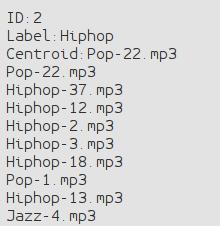
\includegraphics{resources/result11}
        \caption{Result Overview}
        \label{fig:figure7}
\end{figure}
\par The cluster is identified by its ID. We also obtain the initial centroid used by the cluster which is useful in giving us an indication as
to how the clusters were formed and how much impact the initial choice had. Furthermore, each of the clusters are labeled to be one of the five
Genre and this is also part of the output.\\ 
The process of labeling the cluster is discussed in the next section. 

\subsection{Validation Process}
We were uniquely placed in terms of how the validation needed to be carried out. As it was not supervised learning, there was no notion of training and
test dataset distinction. However, it also wasn't one of those (normal) cases where we do clustering in a completely unsupervised manner hoping to discovery new knowledge. Instead, we had true labels of the song genre which could/should be used to validate the results obtained. And so, we needed to perform external evaluation of the clusters as opposed to internal evaluation (Dunn Index, Silhouette coefficient). 
\par Eventually, we settled on using an accuracy measure obtained from the confusion matrix for the five genre. 
\begin{table}[h]
        \caption{Validation Process}
        \label{tab:table1}
        \begin{center}
                \begin{tabular}
                        {|l|l|l|l|l|l|}
                        \hline & Rock & Classical & Pop & Jazz & Hiphop \\ 
                        \hline Rock & \# & - & - & - & - \\ 
                        \hline Classical & - & \# & - & - & - \\ 
                        \hline Pop & - & - & \# & - & - \\ 
                        \hline Jazz & - & - & - & \# & - \\ 
                        \hline Hiphop & - & - & - & - & \# \\ \hline
                \end{tabular}
        \end{center}
\end{table}
\par  The diagonal values of the confusion matrix are the number of correctly assigned songs for each genre. And so, the accuracy is the ratio of the sum
of all diagonal elements to the total number of songs. 
\begin{equation}
        Accuracy(A)=\frac{\sum\limits_{}^{i=j}{M_{ij}}}{\sum\limits_{}^{i,j \in G}{M_{ij}}}
\end{equation}
\par The next job was to determine a way to label each of the clusters as without labeling them we cannot obtain the confusion matrix! To label them we could have simply
labeled the cluster according to which genre holds the majority in the cluster but we found it to be problematic as there might be no clear majority and one
genre might hold a majority in multiple clusters. 
\par Instead, we decided to use a better but computationally expensive approach: try out all possible combinations of the labels and choose the combination with
the best accuracy. Here, we create 120 (5!) possible confusion matrices, calculate the accuracy for each and keep the one with the best result.

\subsection{Results and Discussion}
We used a data-set of 230 songs with the following distribution:\\ 
Pop (40), Rock (50), Classical (50), Jazz (50), Hiphop (40).
\par  The result obtained varies slightly for each run due to the randomness of the initialization process but perhaps due to the small size of the data-set
they usually converge to the same clusters/accuracy. 
\par With all weights ( $w_I$ , $w_M$  and $w_R$ ) set at 1.0; in other words without letting them affect the clustering, we obtain an accuracy of around
46 per cent. 
\par One of the result showing the confusion matrix is given below. This result converged in 16 iterations. The number of iterations vary but mostly
convergence is reached in 10-20 iterations. 
\begin{figure}[h]
        \centering
        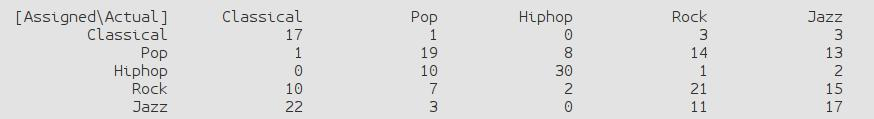
\includegraphics{resources/result22}
        \caption{Cross-Validation}
        \label{fig:figure8}
\end{figure}
\par Each column represents the actual genre of the data-set while each row represents one particular cluster. 
\par As seen from the figure, Hiphop has the best classification with a 75 per cent accuracy. The others don't fare so well with Classical (34 per cent)
being the most badly assigned genre as 22 classical songs has been classified as Jazz.
\begin{figure}[h]
        \centering
        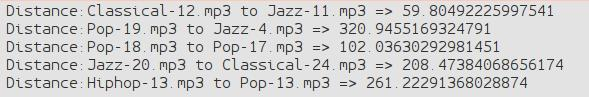
\includegraphics{resources/result33}
        \caption{Inter-cluster Distance}
        \label{fig:figure9}
\end{figure}
\par Initial observations seem to point towards our distance metric being at fault for assuming Classical to be close to Jazz. Or, it could also be
that for the features we have chosen, these two genre are too similar. This problem is also encountered in \cite{Haggblade2011}
\par The system also cannot distinguish Rock, Pop and Jazz from each other with Jazz being classified as Rock being the second biggest problem after
Classical being classified as Jazz. 
\par Overall, as it currently stands, the system is only able to cluster Hiphop songs with satisfactory accuracy. 
